\section{Metode Penelitian}

\subsection{Studi Literatur}
Untuk menunjang pengerjaan penelitian ini, perlu dilakukan studi literatur untuk memberikan pengetahuan yang cukup untuk menyelesaikan penelitian ini. Studi literatur dilakukan dengan cara mengumpulkan dokumentasi dan pustaka yang berkaitan dengan penelitian ini. yaitu:
\begin{enumerate}
    \item Ansible
    \item K3s
    \item Raspberry Pi
\end{enumerate}

\subsection{Tipe Penelitian}
Tipe dari penelitian ini adalah penelitian eksploratif dan implementatif. Dimana akan dilakukan eksplorasi mengenai langkah-langkah yang dapat diambil untuk mengimplementasikan \textit{tech stack} hingga menjadi kluster yang dapat digunakan dalam lingkungan produksi.

\subsection{Rekayasa Kebutuhan}
Tabel berikut menjelaskan setiap kebutuhan yang dibutuhkan untuk melakukan penelitian.
\begin{table}[h]
    \begin{tblr}{
            hlines,
            vlines,
            row{1} = {bg=gray,fg=white,ht=1cm},
            columns = {halign=c},
            colspec = {Q[5cm]},
        }
        \textbf{Proses/ Kebutuhan} & \textbf{Perangkat Lunak/Keras}\\
        Node Master/Slave & Raspberry Pi \\
        Orchestrator & K3s \\
        Automation & Ansible \\
    \end{tblr}
    \centering
    \caption{Tabel kebutuhan penelitian}
\end{table}

\subsection{Rancangan Sistem}
Perancangan sistem dilakukan sebagai tahap awal untuk menggambarkan implementasi sisten secara sistematis dan terstruktur. Hal ini akan dilakukan ketika seluruh rekayasa kebutuhan untuk penelitian telah terpenuhi.
\begin{figure}[htb!]
    \centering
    \begin{tabular}{ @{} r @{} }
        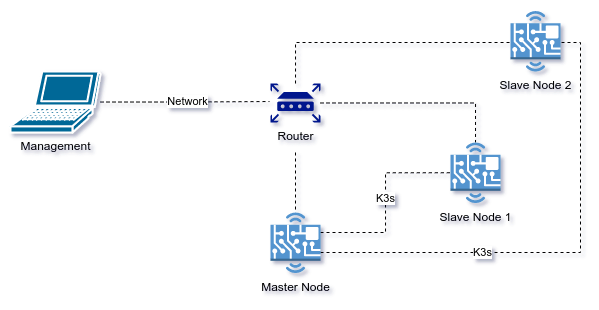
\includegraphics[scale=0.6]{pictures/rancangan_sistem.png}\\
    \end{tabular}
    \caption{Rancangan Sistem}
\end{figure}
\FloatBarrier
\noindent
Dari diagram perancangan diatas, terlihat beberapa node yang berupa Raspberry Pi terhubung pada sebuah router. Dimana router tersebut menghubungkan semua node kepada sebuah komputer manajemen untuk administrasi. Setiap node dapat berkomunikasi dengan node lain melalui Master Node menggunakan K3s dan komputer yang melakukan manajemen dapat mengakses secara langsung setiap node melalui jaringan yang disediakan melalui router.
\subsection{Skenario Pengujian dan Analisis Hasil}
Pengujian dilakukan dengan maksud untuk melihat kinerja sistem dan skalabilitas ketika ditambahkan node baru untuk digunakan oleh K3s dalam melakukan load balancing. Sehingga dapat dilihat efektifitas sistem ketika seluruh node telah menggunakan seluruh sumber dayanya dan memerlukan tenaga komputasi tambahan untuk dapat memproses lebih banyak permintaan.

\subsection{Pembentukan Kesimpulan}
Kesimpulan dibuat ketika informasi dari tahap tahap sebelumnya telah didapatkan dan dapat diringkas untuk membentuk ringkasan dari hasil penelitian.